
\chapter{STATE ESTIMATORS}
\label{chap:Estimators}

Section \ref{chap:StateError} explained the rationale for the state representations and how adjustments can made to them in a manner that preserves the integrity of its connection to the TableSat's physical orientation.  Use of the gains are also investigated with the goal of making gain tuning more intuitive.

\section{State Prediction}
\label{sec:StatePrediction}

Section \ref{sec:BodyRatePIDEstimation} shows that accurate tracking of a spin-stabilized satellite like TableSat or MMS, requires that the body rate dynamics and attitude kinematics/dynamics be coupled.  This is especially important for the NASA MMS TableSat IA implementation since only the magnetometer and coarse sun sensors provide system state feedback.  Furthermore, only a partial measurement of the attitude quaternion is available; there are no direct body rates measurements.

The approach taken in the TSatPy code to create state predictions based upon previous state estimates is to start with a discretized Euler's Moment Equations (\ref{eqn:DiscreteEulerMomentEquations}) to predict $\bs{\dot{\omega}}(t_{k+1})$.  The current estimated body rate is adjusted based on the variable time step size.

\begin{equation}
  \bs{\omega}(t_{k+1}) = \bs{\omega}(t_{k}) + \bs{\dot{\omega}}(t_{k+1})\cdot (t_{k+1} - t_k)
\end{equation}

The newly estimated body rate $\bs{\omega}(t_{k+1})$ is supplied to the discretized quaternion dynamics Equation (\ref{eqn:DiscreteQuaternionPropagation}) to calculate the newly estimated rotational quaternion:

\begin{equation}
  \bs{q}(t_{k+1}) = ( \bs{A} + \bs{B} ) \bs{q}(t_{k}) \\
\end{equation}
where
\begin{equation}
  \begin{aligned}
    \text{where } \bs{A} &= \exp \left( \frac{\Delta t_{k+1}}{2} \bs{\Omega} \left[ \bs{\bar{\omega}}(t_{k+1}) \right] \right)\\
    \bs{B} &= \frac{1}{48} \Delta t_{k+1}^2 \Big(
    \bs{\Omega} \left[\bs{\omega}(t_{k+1}) \right]
    \bs{\Omega} \left[\bs{\omega}(t_{k})   \right] -
    \bs{\Omega} \left[\bs{\omega}(t_{k})   \right]
    \bs{\Omega} \left[\bs{\omega}(t_{k+1}) \right]
      \Big)
  \end{aligned}
\end{equation}


\section{PID State Estimation}
\label{sec:BodyRatePIDEstimation}

This section covers the use of PID adjustments to track state estimation.  The method discussed in Section \ref{chap:StateError} where states and especially the quaternion portion can be scaled can be applied to the proportional term of the PID estimator.

\subsection{Proportional State Estimation}
\label{subsec:ProportionalEstimator}

The proportional estimator defined in Equation (\ref{eqn:PEstimator}) is implemented in TSatPy.  Taking the estimated and measured states from Equation (\ref{eqn:StateDifferenceQuaternionSamples}), an update of the TableSat state estimate is performed in the following manner:

\begin{equation}
  \begin{aligned}
    \bs{\hat{x}}(t_{k+1}) &= \begin{bmatrix} \bs{\hat{q}}(t_{k+1}) \\ \bs{\hat{\omega}}(t_{k+1}) \end{bmatrix} = \begin{bmatrix} \bs{\psi}(\bs{q}_e(t_{k}), K_{qp}) \otimes \bs{\hat{q}}(t_{k}) \\  \bs{\hat{\omega}}(t_{k}) + \bs{K}_{\omega p} \cdot \bs{\omega}_e(t_{k}) \end{bmatrix}
  \end{aligned}
  \label{eqn:PEstimator}
\end{equation}

An example of using a PID controller with TSatPy is shown in Snippet \ref{code:pid_estimator_example}
\begin{listing}[H]
\begin{singlespace}
  \begin{minted}[mathescape,linenos,numbersep=10pt,frame=lines,framesep=2mm]{python}
from TSatPy import StateOperator, Estimator, State
from TSatPy.Clock import Metronome
import numpy as np

x_ic = State.State(
    State.Quaternion([0,0,1],radians=190/180.0*np.pi),
    State.BodyRate([0,0,3]))
print("x_ic:    %s" % (x_ic))

k = 0.2
Kp = StateOperator.StateGain(
    StateOperator.QuaternionGain(k),
    StateOperator.BodyRateGain(np.eye(3) * k))
print("Kp:  %s" % (Kp))

c = Metronome()
pid = Estimator.PID(c, ic=x_ic)
pid.set_Kp(Kp)
print("pid: %s" % (pid))

x_m = State.State(
    State.Quaternion([0,0.1,1],radians=44/180.0*np.pi),
    State.BodyRate([0,0,3.1]))
pid.update(x_m)
print("pid.x_hat:   %s" % (pid.x_hat))

e, r = pid.x_hat.q.to_rotation()
print("e:      <%g, %g, %g>\ndegree: %g" % (
    e[0,0],e[1,0],e[2,0], r * 180.0 / np.pi))

# Prints Out
# x_ic:    <Quaternion [-0 -0 -0.996195], -0.0871557>,
#          <BodyRate [0 0 3]>
# Kp:  <StateGain <Kq 0.2>,
#      <Kw = [[ 0.2 0. 0. ] [ 0. 0.2 0. ] [ 0. 0. 0.2]]>>
# pid: PID
#  x_hat <Quaternion [-0 -0 -0.996195], -0.0871557>, <BodyRate [0 0 3]>
#  Ki None
#  Kp <StateGain <Kq 0.2>,
#     <Kw = [[ 0.2 0. 0. ] [ 0. 0.2 0. ] [ 0. 0. 0.2]]>>
#  Kd None
# pid.x_hat:   <Quaternion [-0.00170765 0.00968454 -0.985915], 0.16696>,
#              <BodyRate [0 0 3.02]>
# e:      <-0.00173196, 0.00982241, -0.99995>
# degree: 160.778
  \end{minted}
\caption{Example of a PID estimator}
\label{code:pid_estimator_example}
\nocite{minted}
\end{singlespace}
\end{listing}

This example demonstrates a proportional estimator initialized to a state of a $190^o$ rotation about $+z$-axis and a body rate of $\omega_z = 3$ rad/sec.  The proportional gain applied to state errors is chosen to be $0.2$ for the quaternion and all body rates.  After the measured state of a $44^o$ rotation about the axis $0 \bs{i} + 0.1 \bs{j} + 1\bs{k}$ and a body rate of $\omega_z = 3.1$ rad/sec is applied, the new estimated state is a $160.778^o$ degree rotation about $0.00173196 \bs{i} - 0.00982241 \bs{j} + 0.99995\bs{k}$ with a body rate of $3.02$ rad/sec.

\begin{figure}[H]
  \centerline{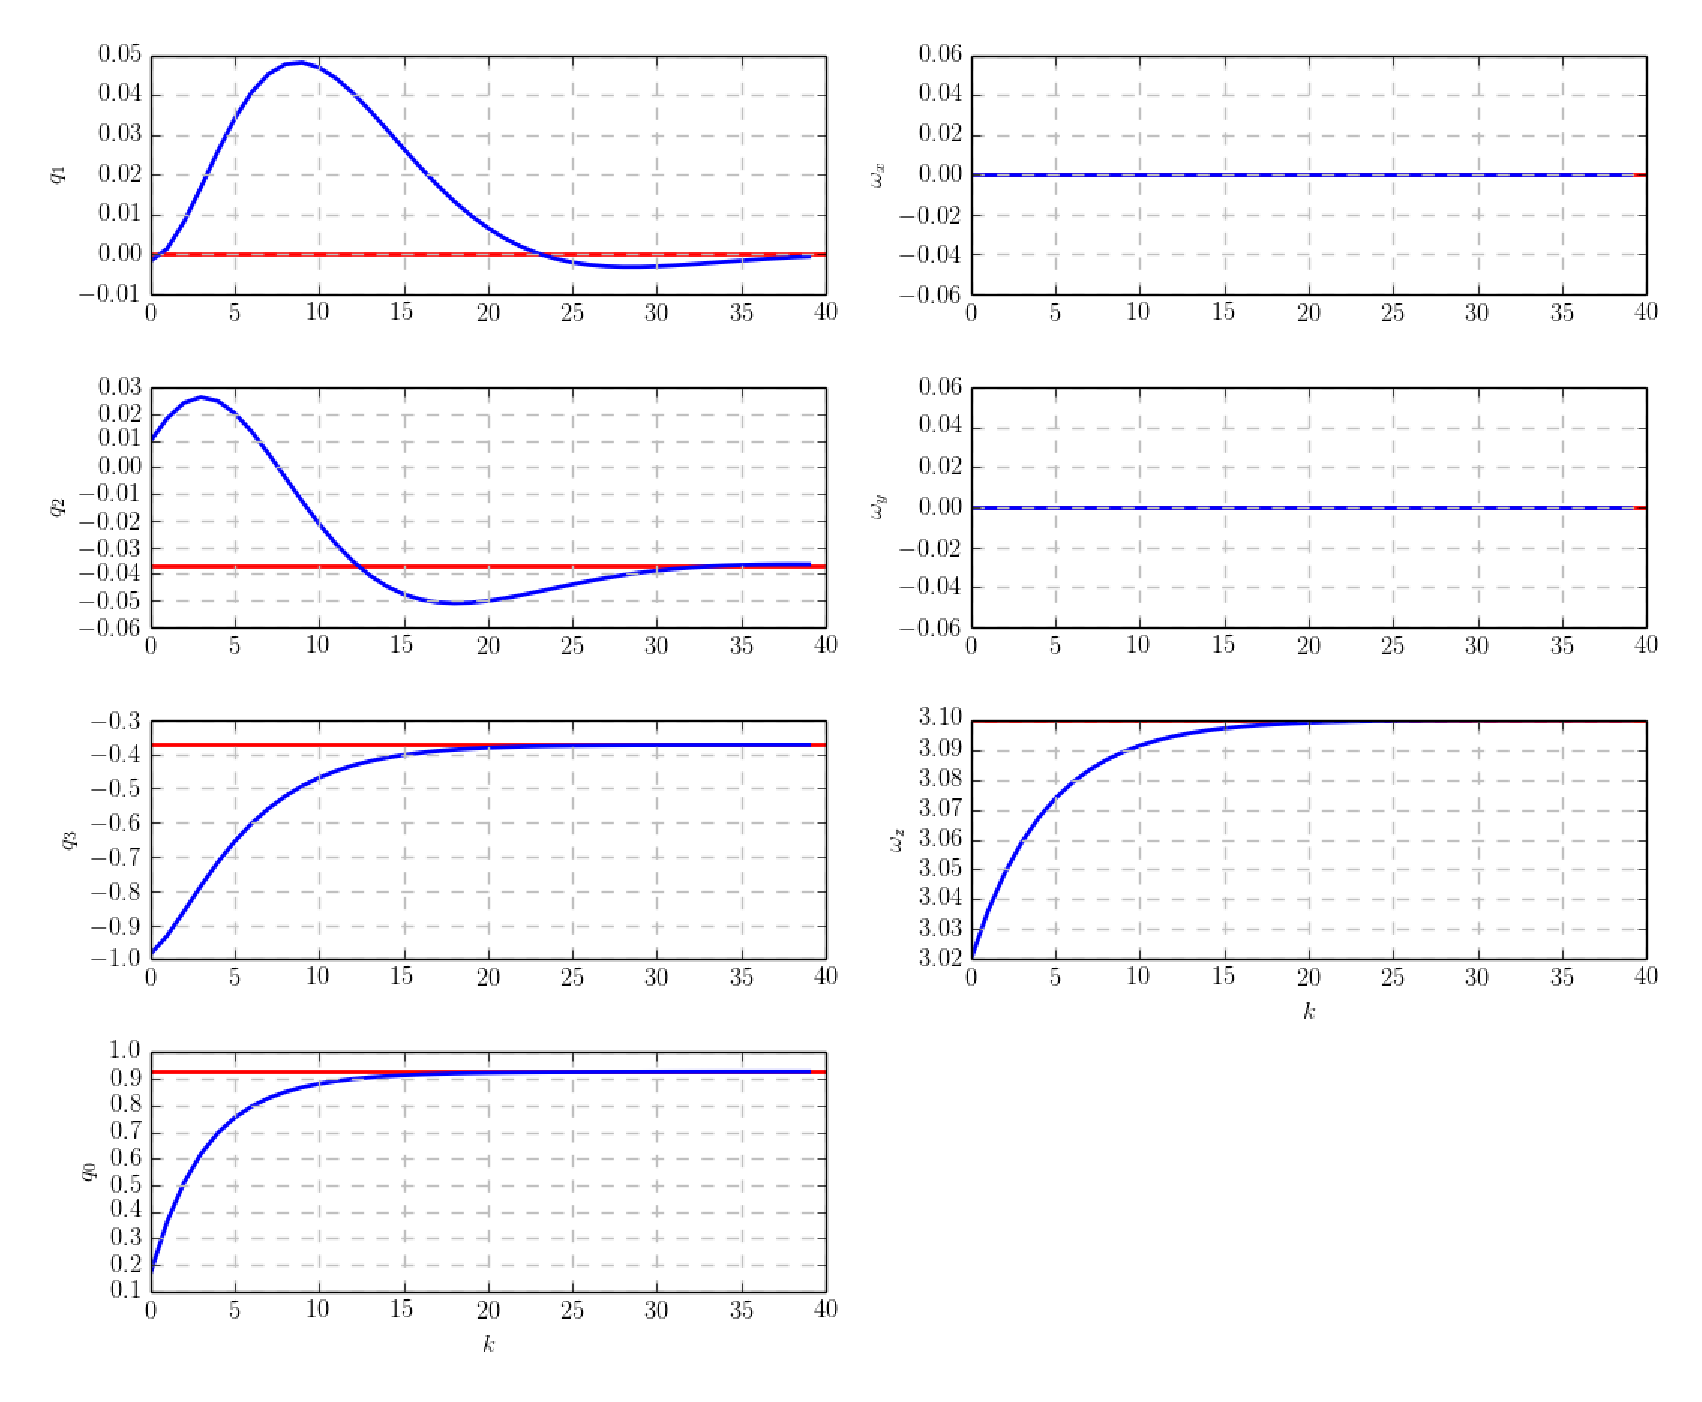
\psfig{file=figures/p_estimator_static_target.eps,width=6in}}
  \caption{P-Estimator state $[\bs{q}\ \bs{\omega}]^T$ with static target}
  \label{fig:PEstimatorwithstatictarget}
\end{figure}

The work covered so far in this chapter assumes the system to be in a static state.  In Figure \ref{fig:PEstimatorwithstatictarget}, a P-Estimator converges its estimated state (blue) to the static measured state (red).  While the estimated state converges to the measured state after about 40 iterations, this type of conversion is effective only for non-rotating systems.  The non-zero $\omega_z$ means that the quaternion attitude representation is in constant motion.

The $3.1$ rad/sec rotation about $0\bs{i} + 0.1\bs{j} + 1\bs{k}$ condition from the previous p-estimator is now allowed to propagate the quaternion state through 10 seconds of rotation with state estimate updates every 0.1 sec.  The resulting measured state (red) and estimated state (blue) is shown in Figure \ref{fig:PEstimatorwithrotatingtarget}.  The body rates track identically to those in Figure \ref{fig:PEstimatorwithstatictarget} where $t(k) = 2$ corresponds to $k = 20$.  Due to having only proportional compensation and no predictive methods, after the initial transient the state estimates exhibit, at best, convergence with steady state error.

\begin{figure}[H]
  \centerline{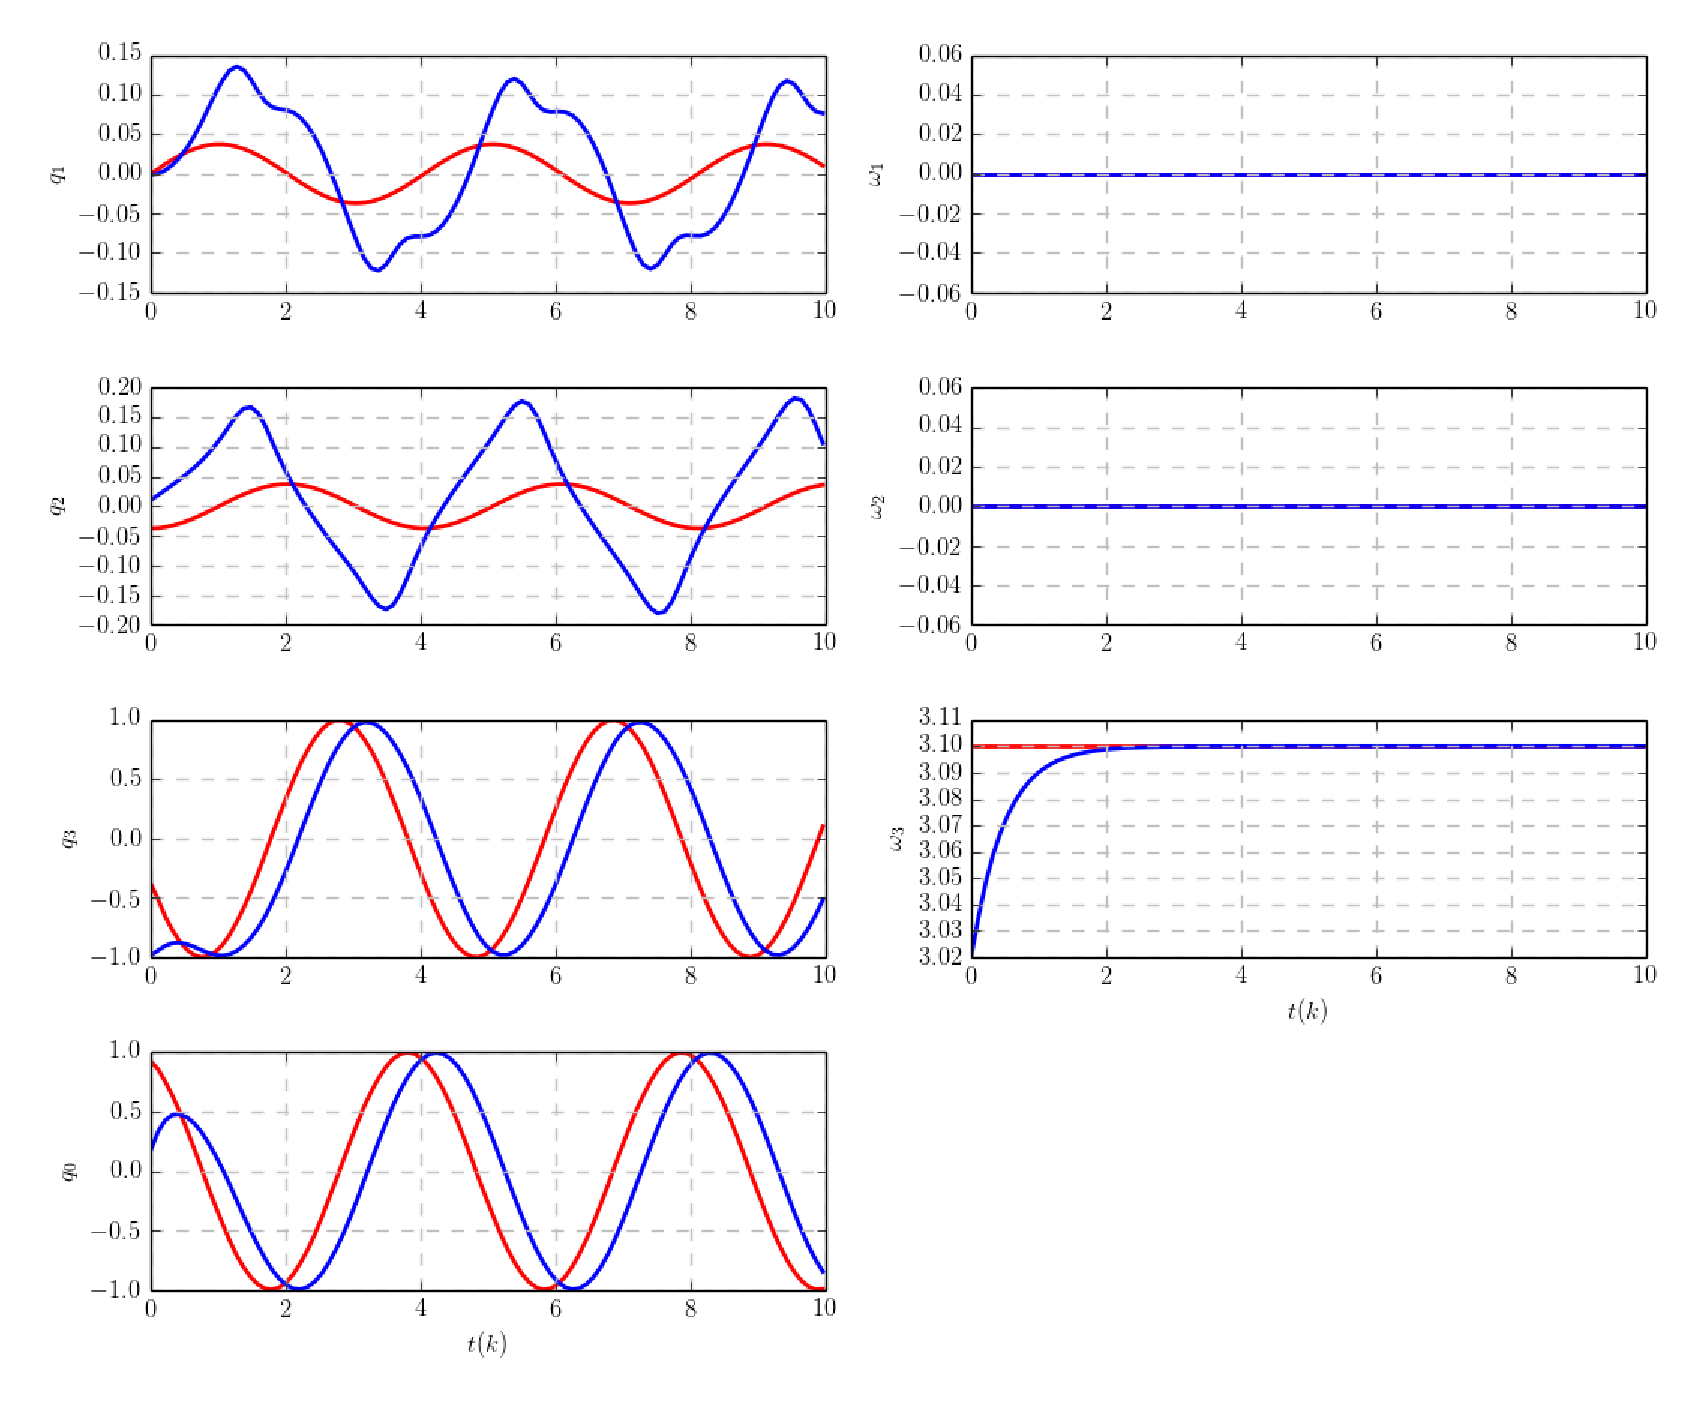
\psfig{file=figures/p_estimator_3radps.eps,width=6in}}
  \caption{P-Estimator state $[\bs{q}\ \bs{\omega}]^T$  with rotating target}
  \label{fig:PEstimatorwithrotatingtarget}
\end{figure}

Increasing the frequency of updates to the p-estimator can decrease the error between the measured and estimated states, but the steady state error will persist.  For better results the estimator needs to take into consideration changes in the state through the PID estimator's integral and derivative terms.

\subsection{Integral State Estimation}
\label{subsec:IntegralEstimator}

To maintain consistency with the findings in Chapter \ref{chap:StateError}, the quaternion portion of the integrated state must abide by the quaternion multiplicative correction method.  This is the first model where the variable time step is also taken into consideration.  Instead of accumulating the error measurements, the error corrections are weighted according to the length of time between updates $t_k$ and $t_{k_1}$.  In a simplified case the integral term should be identical in the following two update instances:
\begin{table}[H]
  \centering
  \begin{tabular}{r|c|c|c|c|c}
    $t_1 (sec)$ & 0.1 & 0.2 & 0.3 & 0.4 & 0.5 \\ \hline
    $\theta_e$ & 4 & -3 & -3 & -3 & 5 \\
    \\
    $t_2 (sec)$ & 0.1 & & & 0.4 & 0.5 \\ \hline
    $\theta_e$ & 4 &  &  & -3 & 5 \\
  \end{tabular}
  \label{tbl:VariableUpdates}
\end{table}
In $t_1$, regular updates occur every 0.1 sec ending in an integral error value of 0.  In $t_2$, not taking into consideration the variable step sizes would end in an error value of $+6$.  Here, the -3 error should weighted by the $0.3$ seconds elapsed since the last update.

Propagating the state estimator without compensating for variations in time step sizes can create inconsistencies between different experimental runs.  In Figure \ref{fig:IEstimatorwithouttimevariationcompensation}, the integral estimator was updated with a fixed state for 30 seconds.  The estimator is initialized at $0$ radians and run three times at a fixed angle of $0.5$ radians.  The first simulation has an estimation update frequency of every 0.4 seconds (blue), the second is updated every 0.1 seconds (red), and the third has a variable update frequency (green) that oscillates between updates of every 0.05 to 0.4 seconds.

\begin{figure}[H]
  \centerline{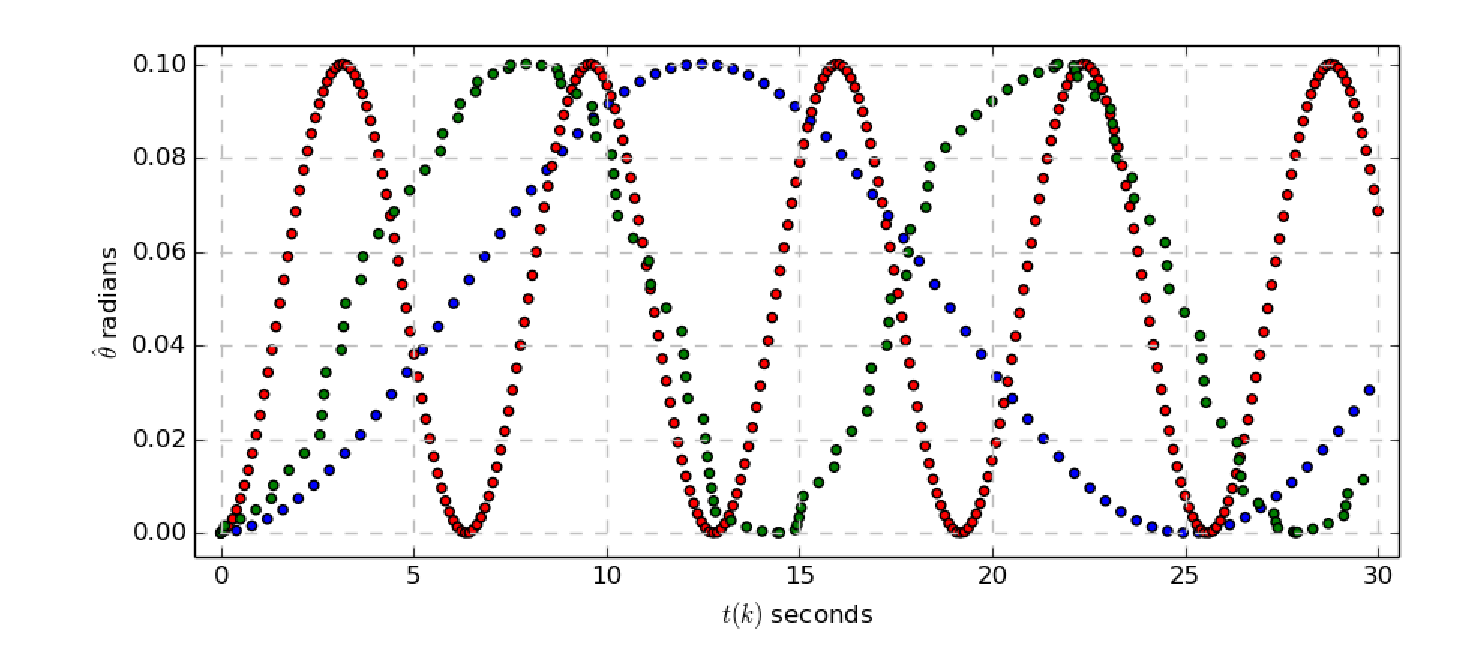
\psfig{file=figures/i_estimator_no_time_varying.eps,width=6in}}
  \caption{I-Estimator without time variation compensation}
  \label{fig:IEstimatorwithouttimevariationcompensation}
\end{figure}

Each calculated estimate for $\hat{\theta}$ in the $k$ domain is identical for each of the three test simulations, but varies greatly in the time domain.  Most notably, the third simulation (alternating between update frequencies) results in an estimation dynamic that could result in a less robust controller.

In comparison, the PID state estimator is modified to incorporate the time step size into its integral term.  The same three tests are run as above with a 0.1 (red), 0.4 (blue), and variable 0.05/0.4 (green) time steps.  The adjustment quaternion method from Section \ref{sec:HighIntegrityStateAdjustments} is first used to compensate for measured time step size of $\Delta t_{k}$ creating a consistent error quaternion.  Then, as used as before, the error quaternion is scaled by a selected gain.  The results of this work can be seen in Figure \ref{fig:IEstimatorwithtimevariationcompensation} where the three tests are still not identical, but their dynamics are more similar than in the previous example.  More notably, the variable step test (green) shows less variability in the estimate being produced.  In a real application, this would reduce any noise being ``transferred'' to the control algorithm.  The resulting state estimate dynamics and error quaternion is
\begin{equation}
  \begin{aligned}
    \bs{\hat{x}}(t_{k+1}) &= \begin{bmatrix} \bs{\hat{q}}(t_{k+1}) \\ \bs{\hat{\omega}}(t_{k+1}) \end{bmatrix} =
    \begin{bmatrix} \bs{\psi}\big(\bs{q}_{ei}(t_k), K_{qi}\big) \otimes \bs{\hat{q}}(t_{k}) \\
     \bs{\hat{\omega}}(t_{k}) + \bs{K}_{\omega i} \cdot (\Delta t_k \bs{I})\cdot \bs{\omega}_e(t_{k}) \end{bmatrix}
  \end{aligned}
  \label{eqn:IEstimator}
\end{equation}
where $\bs{q}_{ei}(t_k) = \bs{\psi}(\bs{q}_e(t_{k}), \Delta t_{k}) \otimes \bs{q}_{ei}(t_{k-1})$.  Here, the error quaternion $\bs{q}_{ei}(t_k)$ is an accumulation of the time step scaled errors encountered in all previous steps.  This is analogous to a ``running sum'' of error values.  For body rate estimation, the traditional integral component with an extra $\Delta t_k \bs{I}$ term is largely responsible for the linear scaling of the body rate error calculations based on the size of the current time step.

\begin{figure}[H]
  \centerline{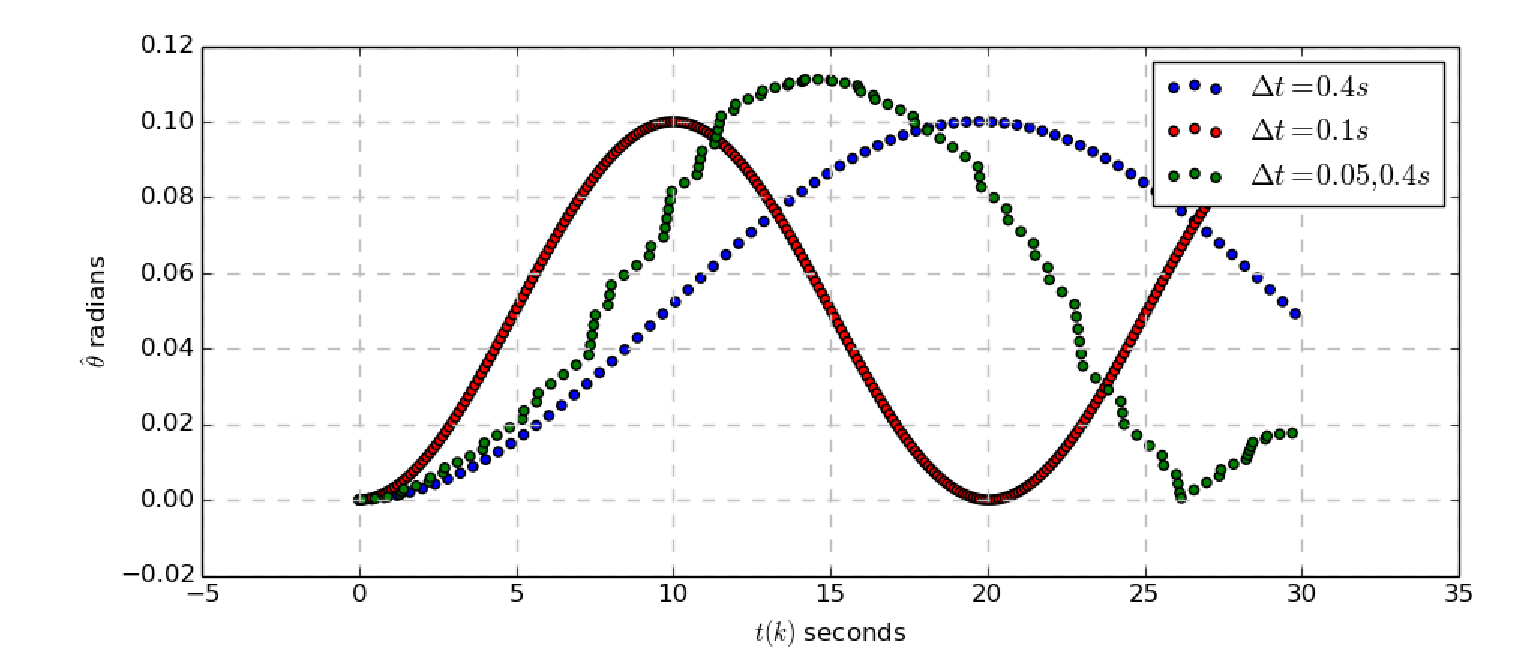
\psfig{file=figures/i_estimator_time_varying.eps,width=6in}}
  \caption{I-Estimator with time variation compensation}
  \label{fig:IEstimatorwithtimevariationcompensation}
\end{figure}

\subsection{Derivative State Estimation}
\label{subsec:DerivativeEstimator}

The derivative component of the PID estimator takes a similar form to the integral component in Equation (\ref{eqn:IEstimator}).  The derivative component is affected only by the current error, previous error, and the current time step size.  As with the integral body rate correction, the derivative correction is scaled by $\frac{1}{\Delta t_k}$ to compensate for variable step sizes such that
\begin{equation}
  \begin{aligned}
    \bs{\hat{x}}(t_{k+1}) &= \begin{bmatrix} \bs{\hat{q}}(t_{k+1}) \\ \bs{\hat{\omega}}(t_{k+1}) \end{bmatrix} =
    \begin{bmatrix} \bs{\psi}\left(\bs{q}_{ed}(t_k), K_{qd}\right) \otimes \bs{\hat{q}}(t_{k}) \\
     \bs{\hat{\omega}}(t_{k}) + \bs{K}_{\omega d} \cdot \left(\frac{1}{\Delta t_k} \bs{I}\right) \cdot \bs{\omega}_e(t_{k}) \end{bmatrix} \\
  \end{aligned}
  \label{eqn:DEstimator}
\end{equation}
where $\bs{q}_{ed}(t_k) = \bs{\psi}\left(\bs{q}_e(t_{k-1})^* \otimes \bs{q}_e(t_{k}), \frac{1}{\Delta t_{k}}\right)$

Figures \ref{fig:DEstimatorwithouttimevariationcompensation} and \ref{fig:DEstimatorwithtimevariationcompensation} are the results of three test runs with the same set update frequencies as with the corresponding integral component (0.1/sec, 0.4/sec, and varied).  For this comparison, the TableSat is simulated under a steady $0.01$ rad/s rotation about the body $+z$-axis to generate a constant rate of change for the quaternion instead of the fixed quaternion in the integral test.  The $\theta_{adj}$ parameter tracked for this test is the angular rotation associated with the $\bs{\psi}\left(\bs{q}_{ed}(t_k), K_{qd}\right)$ quaternion adjustment term.

\begin{figure}[H]
  \centerline{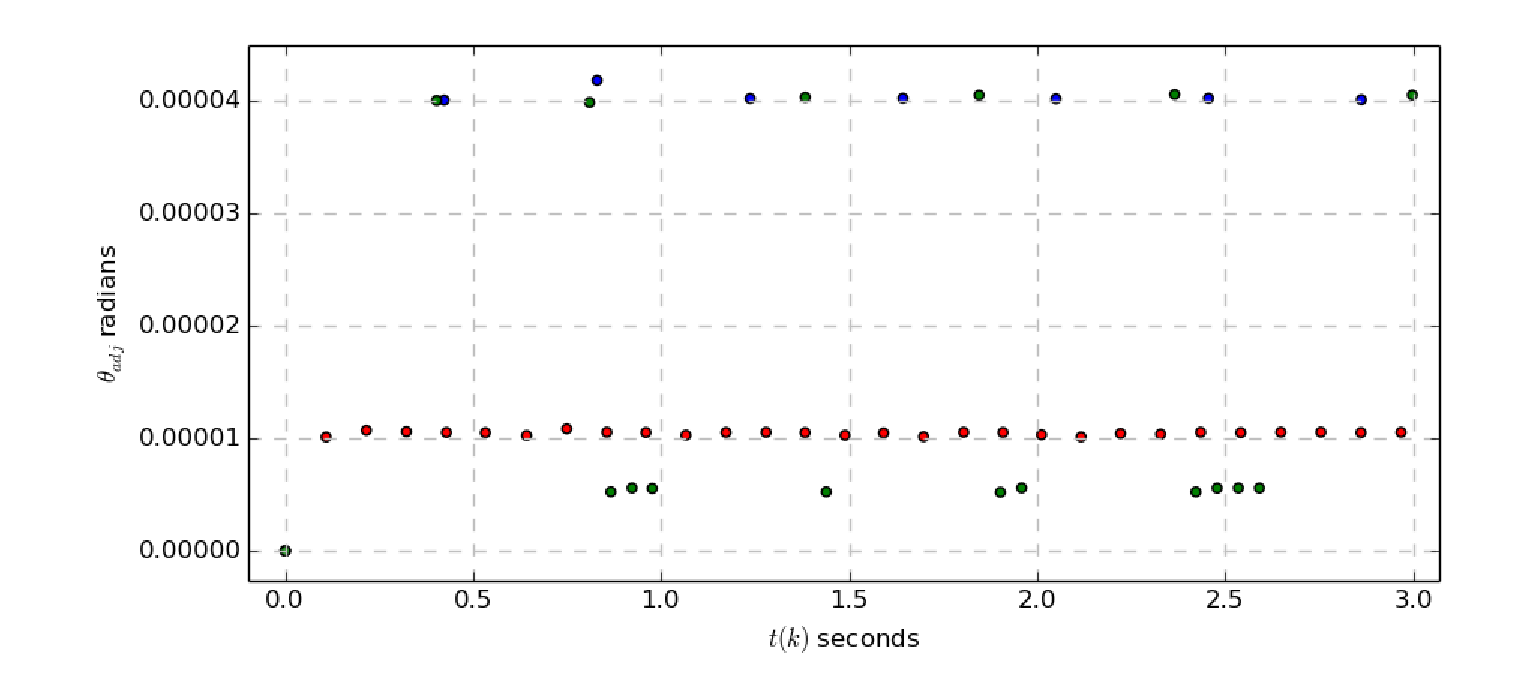
\psfig{file=figures/d_estimator_no_time_varying.eps,width=6in}}
  \caption{D-Estimator without time variation compensation}
  \label{fig:DEstimatorwithouttimevariationcompensation}
\end{figure}

Figure \ref{fig:DEstimatorwithouttimevariationcompensation} shows the results for when time step sizes is not taken into account.  With a constant spin rate, the resulting quaternion adjustment is significantly coupled to the given update frequencies.  The variable time step sequence is a particular concerns as it jumps back and forth between adjusted amount suggesting the spin rate is not constant.

\begin{figure}[H]
  \centerline{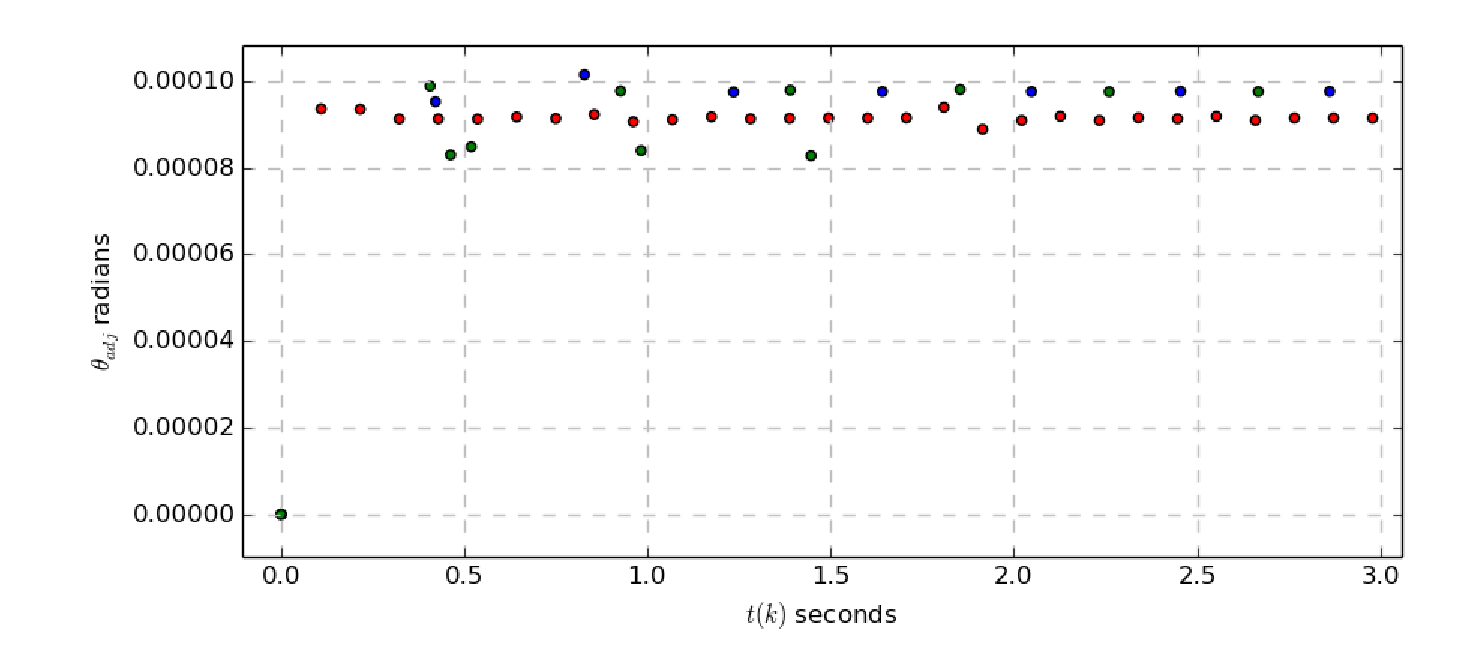
\psfig{file=figures/d_estimator_time_varying.eps,width=6in}}
  \caption{D-Estimator with time variation compensation}
  \label{fig:DEstimatorwithtimevariationcompensation}
\end{figure}

Figure \ref{fig:DEstimatorwithtimevariationcompensation} implements the time variation compensation in Equation (\ref{eqn:DEstimator}) where the quaternion adjustments provides a better representation of the measured constant spin rate.

\subsection{PID State Estimation of Unforced Motion}
\label{subsec:PIDEstimatorofUnforcedMotion}

Combining the proportional, integral, and derivative estimator portions from above, the resulting PID state estimator is as follows:
\begin{equation}
  \bs{\hat{x}}(t_{k+1}) = \begin{bmatrix} \bs{\psi}\left(\bs{q}_{ed}(t_k), K_{qd}\right) \otimes \bs{\psi}\big(\bs{q}_{ei}(t_k), K_{qi}\big) \otimes \bs{\psi}(\bs{q}_e(t_{k}), K_{qp})  \otimes \bs{\hat{q}}(t_{k}) \\
  \bs{\hat{\omega}}(t_{k}) + \bs{K}_{\omega p} \cdot \bs{\omega}_e(t_{k}) + \bs{K}_{\omega i} \cdot (\Delta t_k \bs{I})\cdot \bs{\omega}_e(t_{k}) + \bs{K}_{\omega d} \cdot \left(\frac{1}{\Delta t_k} \bs{I}\right) \cdot \bs{\omega}_e(t_{k}) \end{bmatrix}
  \label{eqn:PIDEstimatorUnforcedMotion}
\end{equation}

The update to the estimated body rate follows the traditional method of the PID controller, the only difference being the addition of the scaling factors for the integral and derivative terms that compensate for non-uniform step sizes.  The quaternion correction is a compilation of the individual correction quaternions and joined through multiplicative error correction.

With a spin-stabilized satellite, controlling the body rate is accomplished with the use of a PID controller.  A test is run through TSatPy based on the PID estimator in Equation (\ref{eqn:PIDEstimatorUnforcedMotion}).  The system is set at a constant spin rate of $0.314$ rad/sec rotation about $+z$ with the measurement of the quaternion angle $\theta$ containing Gaussian noise of $N \sim (0, 0.1218)$ radians.  A gradient descent gain selection settled on the following parameters:
\begin{equation}
  \begin{aligned}
    K_{qp} &= 0.98, K_{qi} = 0.001, K_{qd} = 0.001 \\
    \bs{K}_{\omega p} &= 0.7 \bs{I}, \bs{K}_{\omega i} = \bs{0}, \bs{K}_{\omega d} = \bs{0}
  \end{aligned}
\end{equation}

The test run results are shown in Figure \ref{fig:PIDEstimatorwithoutstateprediction}.  The bottom two graphs show body rate tracking performance where the basic proportional control quickly brings the body rate to desired values.  The quaternion estimators are much more difficult, largely due to the lack of a system model to convert body rates to estimated attitudes at the next update.  Since satellite TableSat IA is spin-stabilized and the estimated quaternion has no prior knowledge of the next value, it relies on a large proportional component to ``jump'' to the new measurement values on each update.

The performance of the integral and derivative components shows an improved performance when incorporating the effects of the variable time step.  However, in this test with such a heavy reliance on the proportional component, the benefits to considering the variable time step effects are negligible.

\begin{figure}[H]
  \centerline{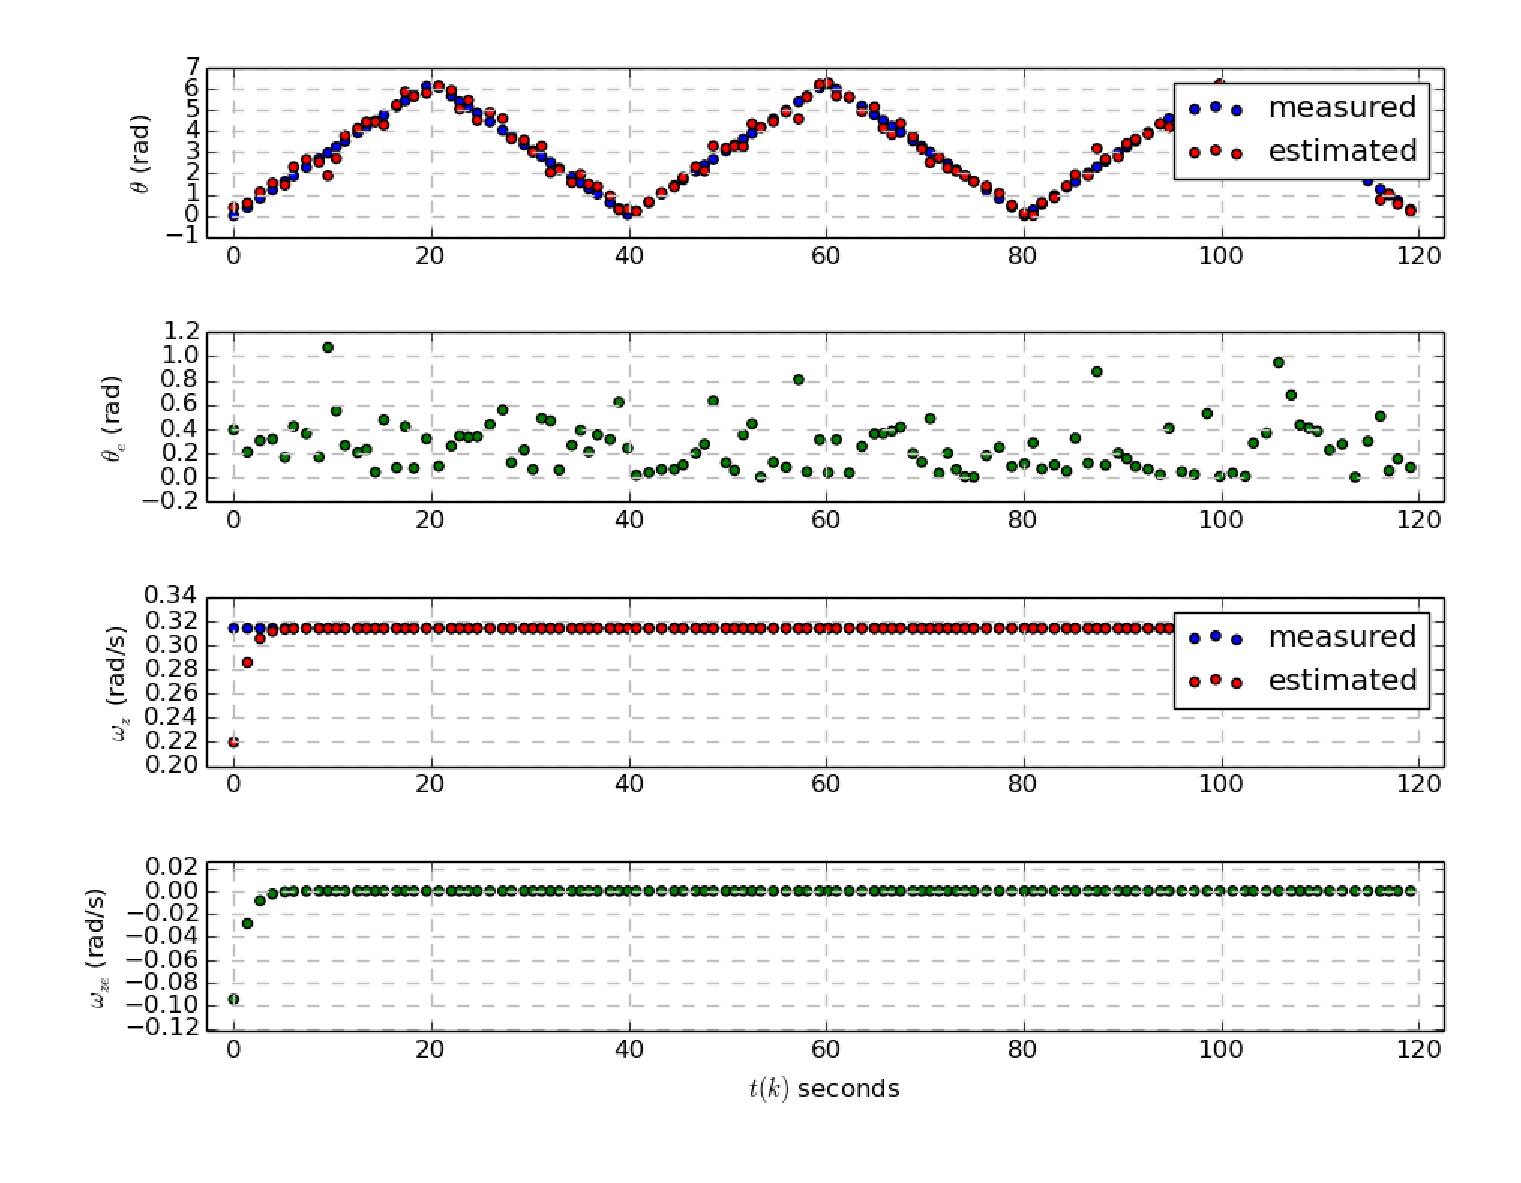
\psfig{file=figures/pid_estimator_no_prediction_high_P.eps,width=6in}}
  \caption{PID-Estimator without state prediction}
  \label{fig:PIDEstimatorwithoutstateprediction}
\end{figure}


\subsection{PID State Estimation with State Prediction}
\label{subsec:PIDEstimatorwithStatePrediction}

From Section \ref{sec:BodyRatePIDEstimation}, Equation (\ref{eqn:PIDEstimatorUnforcedMotion}) defines a method of tracking unforced spin-stabilized satellites through PID state estimation.  The biggest issue is a heavy reliance on the proportional gain to track the quaternion attitude which is sensitive to measurement noise.  Incorporating a multiplicative correction quaternion based model of the TableSat's rigid body dynamics can assist in predicting the $t_{k+1}$ state of the system:

\begin{equation}
  \bs{\hat{x}}(t_{k+1}) = \begin{bmatrix} \bs{\psi}\left(\bs{q}_{ed}(t_k), K_{qd}\right) \otimes \bs{\psi}\big(\bs{q}_{ei}(t_k), K_{qi}\big) \otimes \bs{\psi}(\bs{q}_e(t_{k}), K_{qp})  \otimes \bs{\hat{q}}(t_{k+1})^- \\
  \bs{\hat{\omega}}(t_{k+1})^- + \bs{K}_{\omega p} \cdot \bs{\omega}_e(t_{k}) + \bs{K}_{\omega i} \cdot (\Delta t_k \bs{I})\cdot \bs{\omega}_e(t_{k}) + \bs{K}_{\omega d} \cdot \left(\frac{1}{\Delta t_k} \bs{I}\right) \cdot \bs{\omega}_e(t_{k}) \end{bmatrix}
  \label{eqn:PIDEstimatorwithPredictionUnforcedMotion}
\end{equation}
with the a priori state $\bs{\hat{x}}(t_{k+1})^-$ given as

\begin{equation}
  \bs{\hat{x}}(t_{k+1})^- = \begin{bmatrix}\bs{\hat{q}}(t_{k+1})^- \\ \bs{\hat{\omega}}(t_{k+1})^- \end{bmatrix} = f \Big( \bs{\hat{q}}(t_{k}), \bs{\hat{\omega}}(t_{k}) \Big)
\end{equation}

The PID state estimator now with a state prediction method is simulated again under the same testing conditions present in Figure \ref{fig:PIDEstimatorwithoutstateprediction}.  The resulting performance shows that the inclusion of the system model greatly reduces the reliance on the proportional component of the PID estimator which, in turn, reduces the noise and increases the accuracy of the final estimates being provided to the controller.  The results in Figure \ref{fig:PIDEstimatorwithstateprediction} show the improved quaternion angle estimates, which use the following gains:
\begin{equation}
  \begin{aligned}
    K_{qp} &= 0.0735, K_{qi} = 0.000863, K_{qd} = 0.00812 \\
    \bs{K}_{\omega p} &= 0.7 \bs{I}, \bs{K}_{\omega i} = \bs{0}, \bs{K}_{\omega d} = \bs{0}
  \end{aligned}
\end{equation}
The quaternion's proportional value is still the dominant gain, but has been reduced by 92.5\% of it's previous value while still providing about 80\% reduction in quaternion attitude error rates.

\begin{figure}[H]
  \centerline{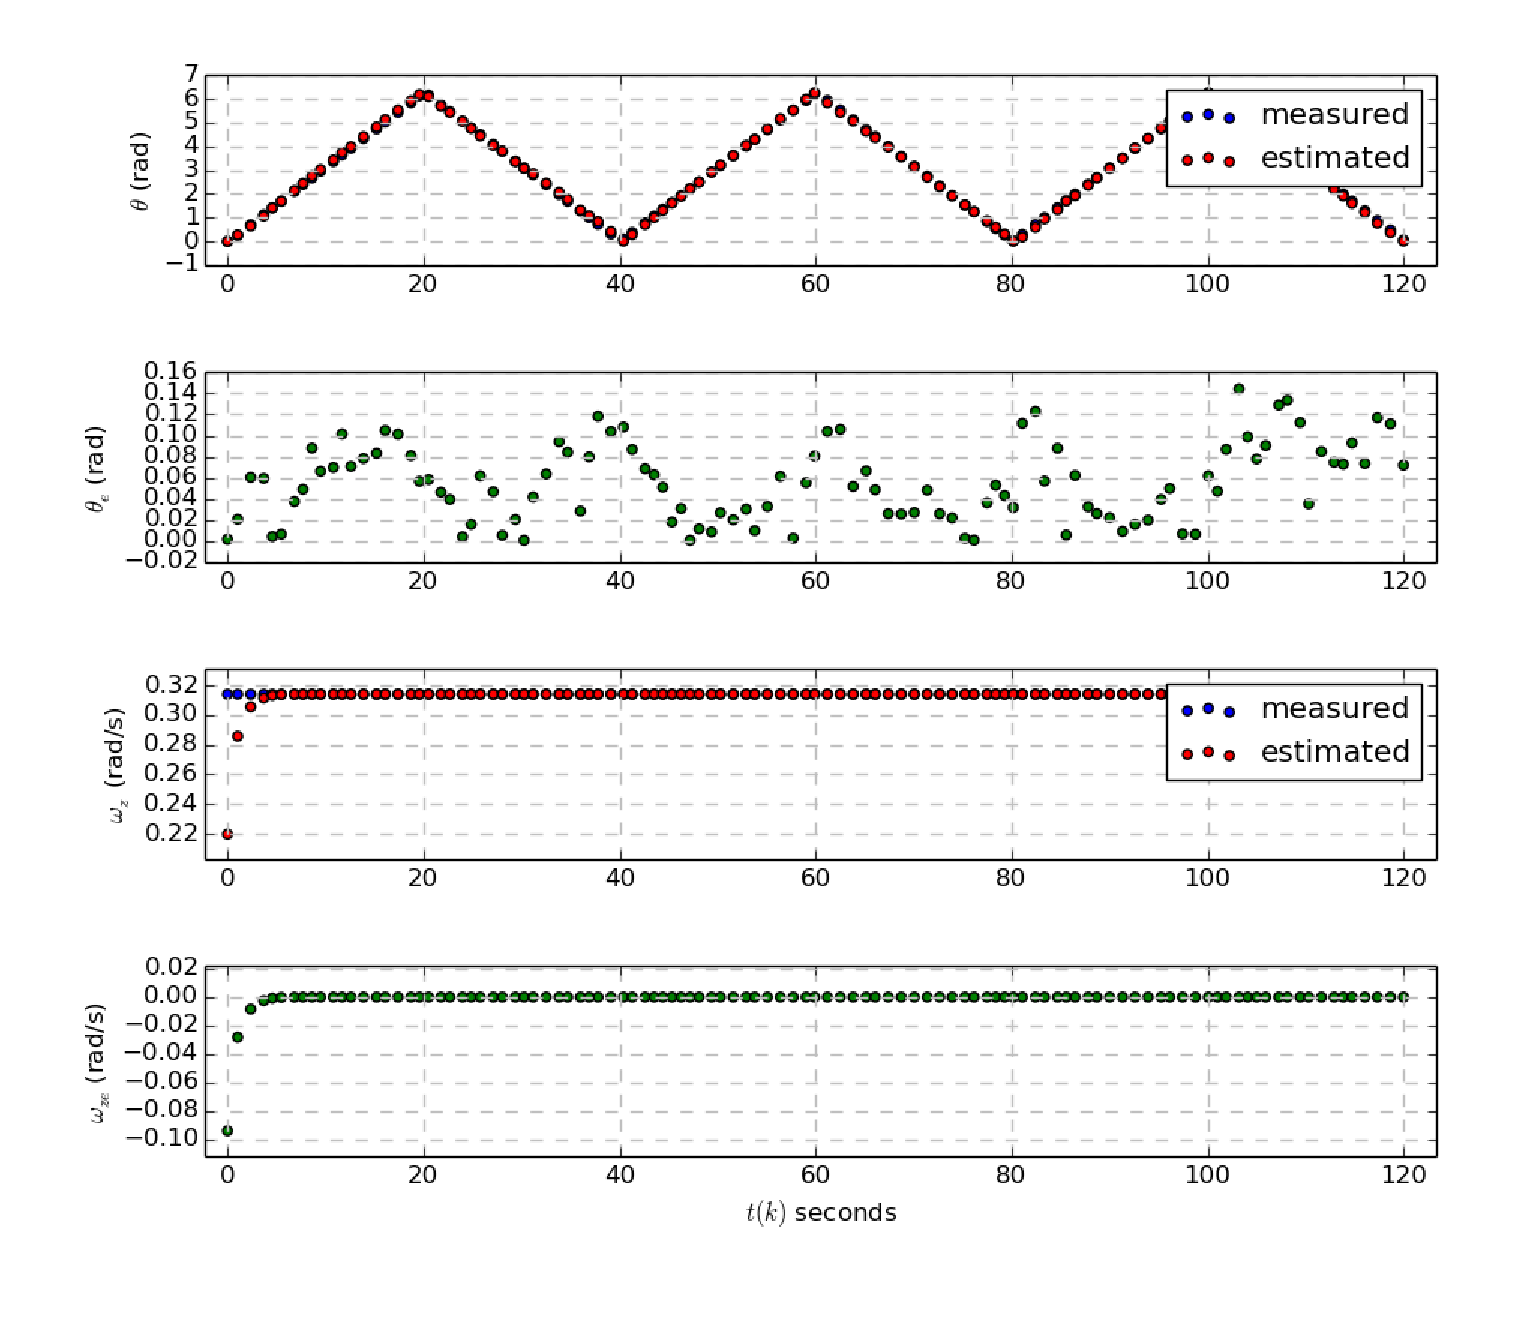
\psfig{file=figures/pid_estimator_with_prediction.eps,width=6in}}
  \caption{PID-Estimator with state prediction}
  \label{fig:PIDEstimatorwithstateprediction}
\end{figure}

\section{Sliding Mode Observer with State Prediction}
\label{sec:SlidingModeObserverwithStatePrediction}

The Sliding Mode Observer (SMO) is a proportional estimator with an additional smoothing term that uses a chosen sliding surface.  The general form for the SMO is
\begin{equation}
  \bs{\dot{\hat{x}}} = \bs{\hat{f}}(\bs{\hat{x}}, \bs{\hat{u}}, t) + \bs{L}(\bs{C}\bs{\hat{x}} - \bs{C}\bs{x}) + \bs{K}\bs{1}_s\bs{\hat{y}}
  \label{eqn:SMOContinuous}
\end{equation}

\begin{figure}[ht]
  \centerline{
\psfig{file=figures/saturation_function.eps,height=1in}}
  \caption{Saturation Function}
  \label{fig:SaturationFunction}
\end{figure}

Where L is a luenberger gain and $\bs{1}_s$ is a switching function.  The sliding mode terms allow additional control of the state adjustments without adding significant computational complexity.  The SMO can continue to use the nonlinear model's state predictions, as in the PID estimators in Section \ref{subsec:PIDEstimatorwithStatePrediction}, which is an advantage over methods such as the Extended Kalman Filter (EKF), where the system is linearized about an operating point and assumes a constant time step.

This thesis takes the discretized form of Equation (\ref{eqn:SMOContinuous}) with a quaternion multiplicative correction:
\begin{equation}
  \bs{\hat{x}}(t_{k+1}) = \begin{bmatrix} \bs{\psi} (\bs{1}_s\big(\bs{q}_{e}(t_k)\big), K_q) \otimes \bs{\psi}(\bs{q}_e(t_{k}), L_{q})  \otimes \bs{\hat{q}}(t_{k+1})^- \\
  \bs{\hat{\omega}}(t_{k+1})^- + \bs{L}_{\omega} \bs{\omega}_e(t_{k}) + \bs{K}_{\omega}\bs{1}_s \big(\bs{\omega}_e(t_{k}) \big) \end{bmatrix}
  \label{eqn:SMOEstimatorwithPredictionUnforcedMotion}
\end{equation}
where
\begin{subequations}
  \begin{align}
    \bs{1}_s\big(\bs{q}_{e}(t_k) \big) &= \begin{bmatrix} \bs{v_e} \\ sat\left( \frac{2\cos^{-1} q_{0e} }{S_{q}} \right) \end{bmatrix} \\
    \bs{1}_s \big(\bs{\omega}_e(t_{k}) \big) &= sat\left( \frac{\bs{\omega}_e(t_{k})}{S_{\omega}} \right) \\
    \bs{L}_{\omega} &= L_\omega \cdot \bs{I} \\
    \bs{K}_{\omega} &= K_\omega \cdot \bs{I}
  \end{align}
\end{subequations}

For body rates, the a priori state provides the predicted body rate $\bs{\hat{\omega}}(t_{k+1})^-$ that is updated by a proportional correctional term $\bs{L}_{\omega} \bs{\omega}_e(t_{k})$, as in the P-Estimator, but has an additional saturation function correction term based on sliding surfaces for the individual body rate errors.  As found in the PID estimator, the proportional estimator for a steady spin-stabilized satellite performs adequately.

Similar to the PID estimator, the quaternion SMO limits its focus to the angular measure of the rotational quaternion.  The sliding surface is taken based on the radian measure.  If the radian measure is below the saturation limit, the quaternion remains unchanged.  If however, the quaternion represents a rotation greater than the saturation limit, a saturated quaternion is created about the same Euler axis but limited to the saturation rotation angle.

Simulating the SMO under the same conditions as that of the PID state estimators, the following parameters are located through an iterative gradient descent method that minimizes the quaternion error angle and standard deviation of the error angle:

\begin{equation}
  \begin{aligned}
    L_q = 0.282 &, L_w = 0.444 \\
    K_q = 0.307 &, K_w = 0.464 \\
    S_q = 0.886 &, S_w = 0.569 \\
  \end{aligned}
\end{equation}

Figure \ref{fig:SMOEstimatorwithstateprediction} shows the result of these tests at these optimized parameters.  The inverted angle measurement in the first graph is an artifact of the non-unique representation of a quaternion attitude.  In this case, the estimated angles are being calculated for rotations about the body's $-z$-axis instead of the $+z$ axis.  This further supports the decision made in Chapter \ref{chap:StateError} to use multiplicative error correction as the second graph shows the correct error values.

Although the SMO in this case is able to traverse the initial transient response well, the steady state quaternion error is almost as high that for the PID state estimator with no state prediction method.  This behavior is due to the high levels of quaternion measurement noise.  With the saturation function, the sliding mode observer is still largely a proportional estimator without the assistance of an integral term to smooth out the noise.

\begin{figure}[H]
  \centerline{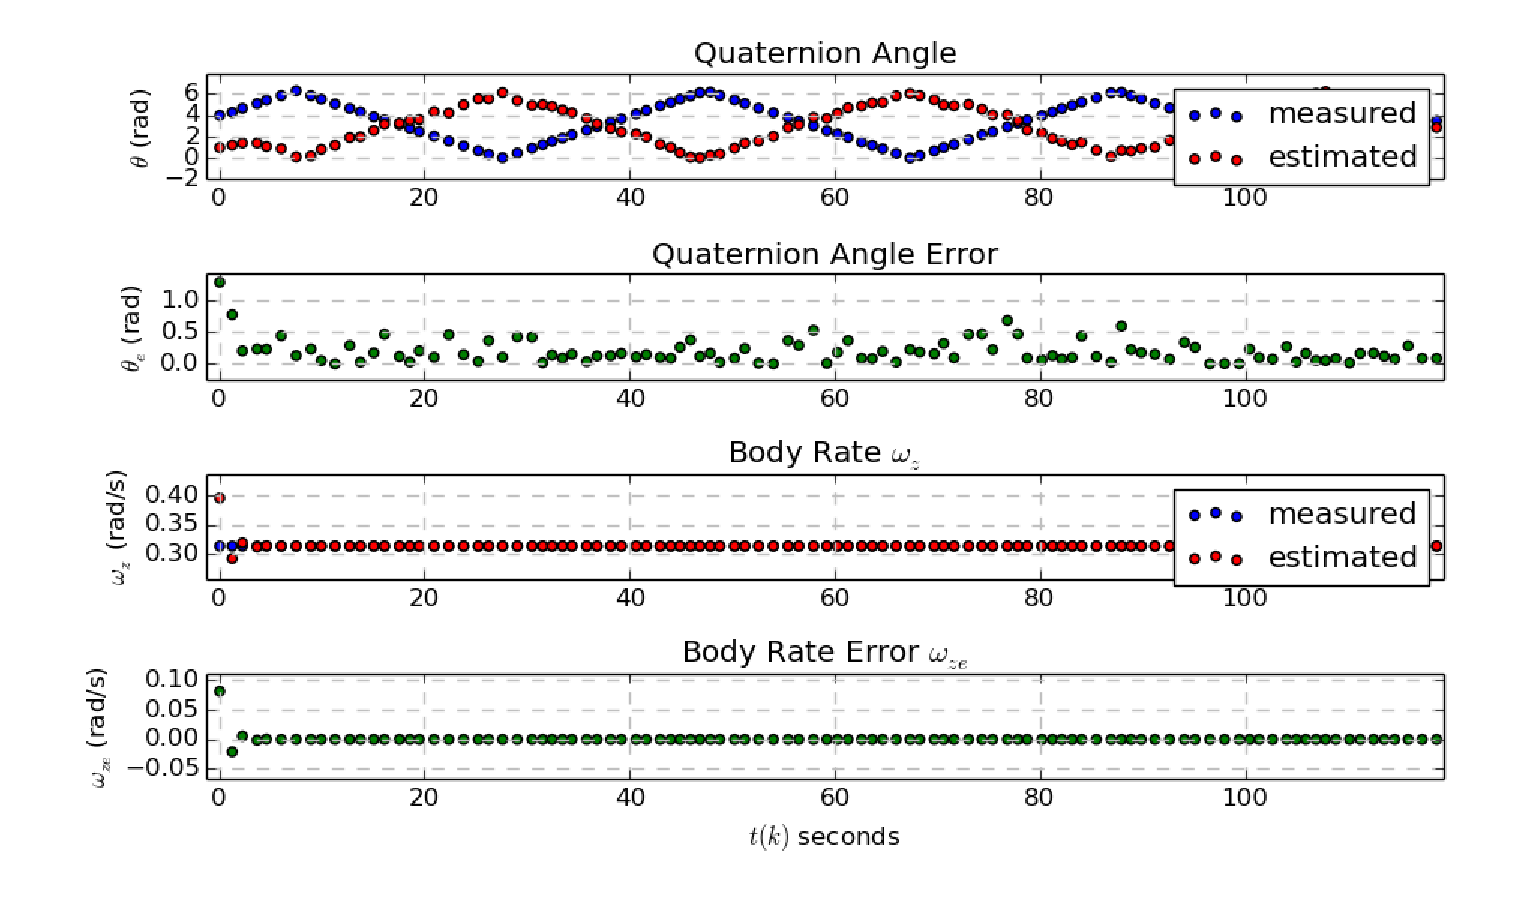
\psfig{file=figures/smo_estimator_with_prediction.eps,width=6in}}
  \caption{SMO-Estimator with state prediction}
  \label{fig:SMOEstimatorwithstateprediction}
\end{figure}

Based on these results, the SMO performs acceptably for body rate estimation.  However, according to the steady state error rates, it appears that PID state estimation is more suitable for steady state attitude tracking.

\section{Comparative Analysis of PID and SMO Estimators}
\label{sec:ComparativeAnalysysofPIDandSMOEstimators}

Both SMO and PID state estimators have similar performance profiles which makes it more complicated to determine the preferred estimation method.  This section discusses how TSatPy can assist with implementing both estimation techniques in parallel to provide a more accurate representation.

One of the advantages of developing the TSatPy code base for the TableSat spin-stabilized is the ability to run a comparative analysis of multiple estimators at the same time.  The estimators run agnostic to the source of the measurements.  In the sample shown below, the state measurements are generated by a model, but can also be switched to use actual TableSat measurement data.

Figure \ref{fig:PIDSMOEstimatorConcurrentComparison} is generated by running a single simulation and providing the truth model's measured state to both a PID and SMO estimator.  This allows for a clear ``side-by-side'' comparison of performance.  Multiple simulations show similar characteristics.  In the initial transient response both estimators are able to converge to a steady state after merely a couple time steps, but the SMO is able to converge slightly faster.  The PID estimator consistently maintains a lower average steady state error but with a slightly higher standard deviation.  As with the initial response, the SMO estimation values generally update slightly just before the PID state estimator.

\begin{figure}[H]
  \centerline{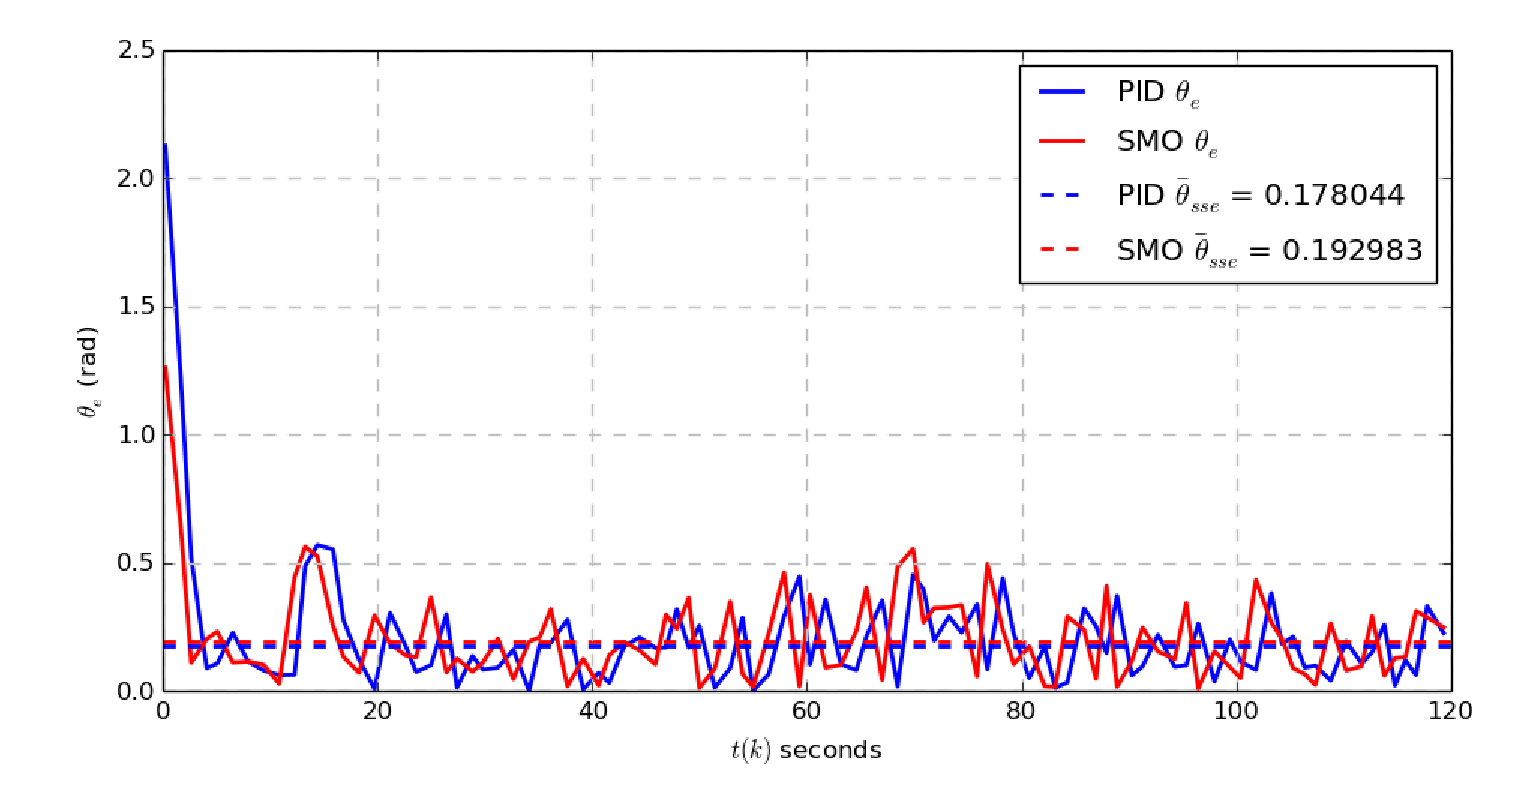
\psfig{file=figures/estimator_comparison.eps,width=6in}}
  \caption{PID/SMO Estimator Concurrent Comparison}
  \label{fig:PIDSMOEstimatorConcurrentComparison}
\end{figure}

The results in Figure \ref{fig:PIDSMOEstimatorConcurrentComparison} are generated through the TSatPy application with the script below.  Lines 10-15 define the two estimators to use in the simulation.  More can be added including the same estimator type with varied parameters.  Lines 17-19 define the system clock behavior.  The simulation run for a simulated 120 seconds as verified in the results above.  The time steps for each update vary between 0.8 and 1.2 seconds randomly.  And since this is running as a simulation instead of obtaining real data from the physical TableSat, the clock rate can be increased to run at 20x speed improving the rate of the iterative testing cycle.

\begin{singlespace}
  \begin{minted}[mathescape,linenos,numbersep=10pt,frame=lines,framesep=2mm]{python}
from TSatPy import Estimator, State
from TSatPy.Clock import Metronome
import numpy as np
import matplotlib.pyplot as plt
import time
import random

print('PID / SMO Estimator Faceoff')

configs = [{'type': 'pid',
 'args': {'kpq': 0.0735,'kpw': 0.7,'kiq': 0.000863,
          'kiw': 0,'kdq': 0.00812,'kdw': 0}
},{'type': 'smo',
 'args': {'Lq': 0.282, 'Lw': 0.444, 'Kq': 0.307, 'Kw': 0.464,
    'Sq': 0.886, 'Sw': 0.569}}]

run_time = 120
speed = 20
dts = [0.8, 1.2]
c = Metronome()
c.set_speed(speed)
I = [[2, 0,  0], [0, 2, 0], [0, 0, 2]]

def setup_estimators(configs):
    x_ic = State.State()
    plant_est = State.Plant(I, x_ic, c)

    est = Estimator.Estimator(c)
    for config in configs:
        est.add(config['type'], plant_est, config['args'])

    return est

def run_comparison(est):
    x_ic = State.State(
        State.Quaternion([0,0,1], radians=4),
        State.BodyRate([0,0,0.314]))
    plant = State.Plant(I, x_ic, c)

    ts = []; smo_err = []; pid_err = []
    start_time = c.tick()
    end_time = c.tick() + run_time
    while c.tick() < end_time:
        plant.propagate()
        offset = np.random.randn() * 20 / 180.0 * np.pi
        q_noise = State.Quaternion([0,0,1], radians=offset) * plant.x.q

        x_m = State.State(q_noise, plant.x.w)

        est.update(x_m)
        ts.append(c.tick() - start_time)

        for model in est.estimators:
            q_e = State.QuaternionError(model.x_hat.q, plant.x.q)
            e, r = q_e.to_rotation()

            if type(model) is Estimator.PID:
                pid_err.append(r)
            elif type(model) is Estimator.SMO:
                smo_err.append(r)
        random.shuffle(dts)
        time.sleep(dts[0] / float(speed))

    return ts, pid_err, smo_err

def graph_it(ts, pid_err, smo_err):
    # Generate the graph here
    # See appendix for the full script

def main():
    est = setup_estimators(configs)
    graph_it(*run_comparison(est))
    return 0

if __name__ == '__main__':
    exit(main())
  \end{minted}
\nocite{minted}
\end{singlespace}

The NASA MMS TableSat IA controller has performance requirements based upon NASA MMS's mission parameters.  It is demonstrated that multiple estimators can be implemented in parallel during both simulations and experimental runs.  As discussed above, this allows better insight into performance differences in estimation methods.  An additional benefit to running the controller through TSatPy is the ability to perform estimator scheduling.  Like gain scheduling, for which an estimator or controller can modify its gains depending on current performance, estimator scheduling allows for switching between disparate estimation techniques during run-time.  For example, one could us an estimator tuned for responding to large errors and have it run along side an estimator tuned for steady state performance.  The control algorithm can then receive more accurate state estimates on a wider range of environmental conditions.
